\section{Algoritmo Exacto}
De acuerdo a lo ya explicado en el inciso \ref{caballitos}, podemos establecer una analog\'ia con este problema y ``El se\~nor de los caballos''. Por lo tanto, la metodolog\'ia empleada para la implementaci\'on del algoritmo exacto tambi\'en fue la de \emph{Backtracking}.\\

De este modo, nos vemos obligados a recorrer inteligentemente todos los conjuntos dentro del conjunto de partes del total de nodos $V$. Mediante el backtracking podemos realizar podas y estrategias para saltear algunas ramas de decisi\'on donde se predice que no se va a poder encontrar la soluci\'on \'optima all\'i.


\subsection{Explicaci\'on y mejoras}
%Explicar detalladamente el algoritmo implementado. Elaborar podas y estrategias que permitan mejorar los tiempos de resolucion.

Nuestro algoritmo recorre ordenadamente el conjunto de partes de V y por cada uno de ellos verifica que cumpla la funci\'on  \texttt{esIndependienteMaximal()}. La misma devuelve 0 si es falso, la cantidad de nodos en el conjunto en caso contrario.

Es decir, se itera sobre los nodos y, considerando el nodo actual como presente o como ausente, termina encontrando el m\'inimo conjunto independiente maximal.\\

En una variable se acumula la soluci\'on \'optima hasta el momento, la cual se actualiza cuando se encuentra un nuevo conjunto independiente maximal que tiene un cardinal menor al \'optimo actual. 
En ella va a quedar la soluci\'on buscada luego de correr el algoritmo.\\

La poda que implementamos consisti\'o en verificar que una futura soluci\'on posible no cuente con una cantidad igual o superior de nodos que la soluci\'on \'optima obtenida hasta el momento. 
Esto quiere decir que si la \'optima actual consiste de $k$ nodos y nos encontramos ante la pregunta de agregar un nuevo nodo a una posible soluci\'on de $k - 1$ nodos, \'esta ser\'a a lo sumo 
tan buena como la que ya ten\'iamos, por lo que no nos resulta \'util contemplarla. De esta forma, se descartan r\'apidamente todas las soluciones peores o iguales que la actual.
\textcolor{red}{... completar}

Y las estrategias fueron \textcolor{red}{... completar}\\

Poner el pseudocodigo...

\begin{algorithm}[h!]
\caption{algoritmo exacto}

\textit{unsigned int} \textbf{calcularCIDM}(Matriz\& \textit{adyacencia}, unsigned int \textit{i}, vector$<$unsigned int$>$\& \textit{conjNodos}, vector$<$unsigned int$>$\& \textit{optimo})\{ 
\newline

\If{(conjNodos.esIndependienteMaximal())}{
		optimo $\longleftarrow$ conjNodos;\\
		\textbf{return} optimo.size();
}
\If{(i.estaEnRango())}{
	\If{(conjNodos es m\'as grande que el optimo actual)}{
		\textbf{return} 0;
	}
	siNoAgrego $\longleftarrow$ calcularCIDM(adyacencia, i+1, conjNodos, optimo);\\
	agrego el nodo $i$ a conjNodos;\\
	siAgrego $\longleftarrow$ calcularCIDM(adyacencia, i+1, conjNodos, optimo);\\
	elimino el nodo $i$ de conjNodos;\\
	\textbf{return} el mejor entre $siNoAgrego$ y $siAgrego$;
}
\textbf{return} 0;
\end{algorithm}

\subsection{Complejidad Temporal}
%Calcular el orden de complejidad temporal de peor caso del algoritmo.
Al ser un algoritmo de $Backtracking$ o fuerza bruta, tiene una complejidad exponencial. En este caso, la misma es de $O(2^n)$, siendo $n$ la cantidad de nodos del grafo. \\

Se llega a dicha complejidad dado que para cada nodo, tenemos que preguntarnos qu\'e ocurre, tanto si lo agregamos al conjunto como si no.\\

Dicho de otra forma, vamos a recorrer todos los conjuntos dentro del conjunto de partes del total de nodos de $V$. El cardinal de dicho conjunto de partes es $2^n$. \textcolor{red}{demostrar o no hace falta?}\\

Para cada uno de los subconjuntos, el algoritmo verifica si cumple la funci\'on \texttt{esIndependienteMaximal()}, la cual
tiene una complejidad en peor caso de $O(n^2)$.	De esta forma, nuestro algoritmo tiene complejidad $O(2^n * n^2)$, lo que es igual a $O(2^n)$.\\

Al tener en cuenta la poda utilizada, se puede ver que la misma no disminuye la complejidad te\'orica planteada dado que en el peor caso, podr\'ia haber que recorrer completamente el conjunto de partes.
De todas formas, dicha poda mejora notablemente los tiempos de ejecuci\'on del algoritmo, como veremos m\'as adelante, ya que descarta las soluciones peores que la \'optima hasta el momento.


\subsection{Experimentaci\'on}
%Realizar una experimentacion que permita observar los tiempos de ejecucion del algoritmo en funcion de los parametros de la entrada y de las podas y/o estrategias implementadas.
Para realizar la experimentaci\'on, se genereron grafos espec\'ificos, que nos permitieron ver el funcionamiento de nuestro algoritmo.
Las conexiones entre los nodos de cada grafo son aleatorias, pero respetando la cantidad de ejes que nosotros definamos previamente.\\

Las instancias con tiempos de ejecuci\'on bajos fueron corridas 100 veces, obteni\'endo luego un promedio de todas, con el fin de eliminar outliers.
Aquellas instancias que tardaban mucho m\'as tiempo, determinamos que los outliers no modificaban en forma considerable, por lo que no nos pareci\'o necesario realizarlas reiteradas veces.\\

\subsubsection{Mejor caso}
De acuerdo a c\'omo fue planteado nuestro algoritmo, se puede ver que el mejor caso posible ser\'a cuando los grafos pasados por par\'ametro sean completos.
Esto es as\'i debido a la poda implementada, ya que cuando considera el primer nodo, ya encuentra una posible soluci\'on y luego descarta r\'apidamente todas las dem\'as, ya que una soluci\'on con un solo nodo ya es una de las \'optimas.\\

\textcolor{red}{Tabla}

  \begin{figure}[h!]
   \begin{center}
 	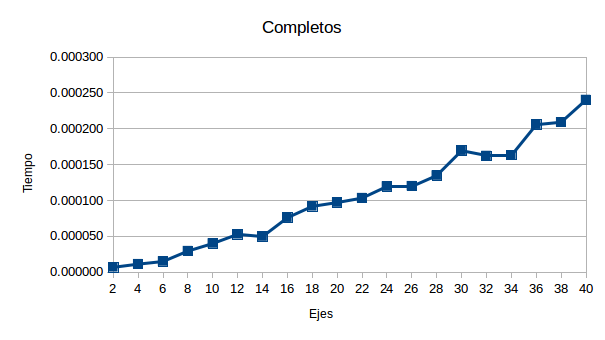
\includegraphics[scale=0.7]{imagenes/exacto/Completos.png}
% 	\caption{}
	\label{GrafoCompleto}
   \end{center}
 \end{figure}

Se puede ver que el gr\'afico tiende a una recta, lo que era esperable ya que encontrar\'a la soluci\'on en el primer nodo, pero luego deber\'a descartar los siguientes $n$ nodos, teniendo una complejidad de $O(n)$.\\

\newpage

\subsubsection{Nodos fijos}
Para continuar viendo el comportamiento del algoritmo, decidimos realizar experimentos fij\'ando la cantidad de nodos y variando la cantidad de ejes.\\
Los tiempos de ejecuci\'on para nodos fijos en 10, 20 y 30 fueron los siguientes:\\
\textcolor{red}{TABLA}

  \begin{figure}[h!]
   \begin{center}
 	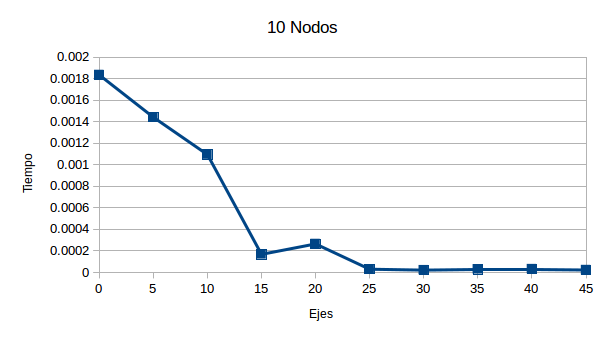
\includegraphics[scale=0.4]{imagenes/exacto/10Nodos.png}
% 	\caption{}
	\label{10Nodos}
   \end{center}
 \end{figure}

  \begin{figure}[h!]
   \begin{center}
 	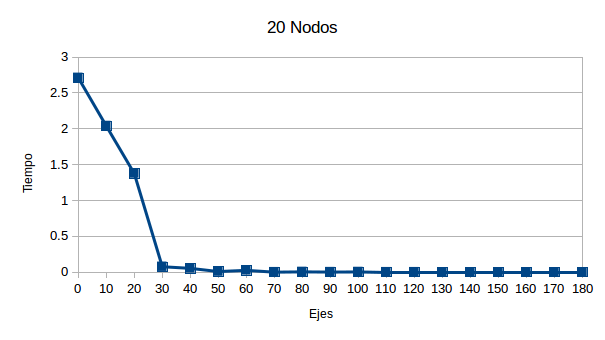
\includegraphics[scale=0.4]{imagenes/exacto/20Nodos.png}
% 	\caption{}
	\label{20Nodos}
   \end{center}
 \end{figure}
   \begin{figure}[h!]
   \begin{center}
 	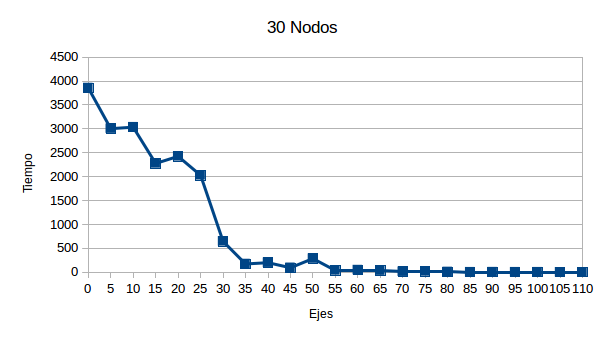
\includegraphics[scale=0.4]{imagenes/exacto/30Nodos.png}
% 	\caption{}
	\label{30Nodos}
   \end{center}
 \end{figure}
 
Como podemos ver, en todos los casos ocurre algo similar: cuando no tienen ejes la ejecuci\'on es m\'as lenta, ya que debe recorrer todas las posibles opciones del conjunto de partes, sin lograr descartar ninguna.
A medida que se van agregando ejes, los tiempos van decreciendo y tienden a ser m\'as lineales, ya que gracias a la poda, no es necesario recorrer todas las posibles soluciones.